\documentclass[a4paper,oneside,12pt]{article}

\usepackage[USenglish]{babel} %francais, polish, spanish, ...
\usepackage{helvet}
\usepackage[T1]{fontenc}
\usepackage[ansinew]{inputenc}

\usepackage{lmodern} %Type1-font for non-english texts and characters

\usepackage{amsmath}
\usepackage{amsthm}
\usepackage{amsfonts}
\usepackage{graphicx}
\usepackage{subcaption}
\usepackage{tabularx}


\usepackage{tikz}
\usepackage{tikz-qtree}
\usepackage{environ}

\makeatletter
\newsavebox{\measure@tikzpicture}
\NewEnviron{scaletikzpicturetowidth}[1]{%
	\def\tikz@width{#1}%
	\def\tikzscale{1}\begin{lrbox}{\measure@tikzpicture}%
		\BODY
	\end{lrbox}%
	\pgfmathparse{#1/\wd\measure@tikzpicture}%
	\edef\tikzscale{\pgfmathresult}%
	\BODY
}
\makeatother


\begin{document}
\fontsize{80}{100}
\fontfamily{phv}
\selectfont 
\noindent
{\bf SWEN 303\\
\fontsize{36}{50}
\selectfont 
Assignment 01\\
\begin{tabularx}{\textwidth}{X| X}
Names & Student IDs\\ \hline
Daniel Medyckyj-Scott & 300336337\\
Alex Ziller & 300414405
\end{tabularx}
}
\pagebreak

\fontsize{12}{14}
\selectfont

\section{Process}

\pagebreak
\section{Model}
\subsection{Overview}
Persons that most likely will use the website
\begin{itemize}
	\item Current students
	\item Potential students
	\item Industry partners
\end{itemize}

\begin{center}
	
\begin{scaletikzpicturetowidth}{\textwidth}
	\begin{tikzpicture}[scale=\tikzscale,
	level distance=5cm]
	
	\Tree[.{Most likely users of website}  
	\edge node{} ; [.{Current students}  
		\edge node{} ; [.{Personae 1} 
			\edge node{} ; [.{Scenario 1} ] 
			\edge node{} ; [.{Scenario 2} ] 
			\edge node{} ; [.{Scenario 3} ] 
			 ] ] 
	\edge node{}; [.{Potential students}    
		\edge node{} ; [.{Personae 2} 
			\edge node{} ; [.{Scenario 1} ] 
			\edge node{} ; [.{Scenario 2} ] 
			\edge node{} ; [.{Scenario 3} ] 
		] 
	] 
	\edge node{}; [.{Industry partners}   
		\edge node{} ; [.{Personae 3} 
			\edge node{} ; [.{Scenario 1} ] 
			\edge node{} ; [.{Scenario 2} ] 
			\edge node{} ; [.{Scenario 3} ] 
		] 
	]
	]

%\Tree[.{Most likely users of website}
%\edge node[midway,left] {false}; [.{Current students}]
%\edge node[midway,right] {true}; [.{Potential students}]
%]
	
	\end{tikzpicture}
\end{scaletikzpicturetowidth}
\end{center}



\pagebreak
%
%\subsection{Personae}
%\subsubsection{Persona1 (Current student)}
%\begin{itemize}
%	\item 21 years old
%	\item 2nd year CompScience student
%	\item Likes using command line for simplest stuff
%	\item Has blue long hair
%	\item In his spare time he writes javascript apps that noone besides him will ever use
%\end{itemize}
%
%\pagebreak
%\subsubsection{Persona2 (Potential student)}
%\begin{itemize}
%	\item 17 years old
%	\item She is good in math but would also like to do something social
%	\item Her friends are all very girly
%	\item She plays football
%	\item She spends her evenings on facebook
%\end{itemize}
%
%\pagebreak
%\subsubsection{Persona3 (Industry partners)}
%\begin{itemize}
%	\item Working at some big software company
%	\item Has already 20 years of professional experience
%	\item Wants to find out new ways of doing a task
%	\item Company can't afford own research
%\end{itemize}
%
%\pagebreak

\subsubsection{Persona 1: Kenneth Smith}
Our nerdy Computer Science student...

\begin{figure}[h]
	\centering
	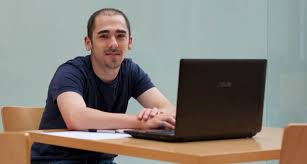
\includegraphics[width = 0.75\textwidth]{images/index.jpg}
\end{figure}
\noindent
\textbf{Personal: }\\
\begin{tabularx}{\textwidth}{l X}
	Name & Kenny\\
	Age & 21\\
	Gender & Male\\
	Education & NCEA Level 3 with Excellence Endorsed (Maths, Chemistry, Digital Technology and Music)\\
	Spare time & PC Gamer (League of Legends, Counter Strike, WoW)\\
	& Heavy metal guitar enthusiast (both plays and listen)\\
	& long distance girlfriend\\
	Attitudes & Considers himself a realist, is more likely a pessimist. Likes to think he knows more than others. Prides himself on his computer abilities so is particularly short tempered  if he is struggling to achieve easy tasks on the computer\\
	Aptitudes & Kenny is intelligent and good at abstract thought.
\end{tabularx}
\noindent
\textbf{Technical: }\\
\begin{tabularx}{\textwidth}{l X}

\end{tabularx}

\pagebreak

\subsection{Scenarios}

\begin{itemize}
	\item asdf
\end{itemize}

\begin{enumerate}
	\item asdf
\end{enumerate}

\end{document}